\documentclass{report}
%Math Stuff
\usepackage{amsmath}
\usepackage{enumitem}
\usepackage{mathtools}

%General Formating
\usepackage[letterpaper, portrait, margin=1in]{geometry}
\usepackage{fancyhdr}
\pagestyle{fancy}

%Bibliography
\usepackage[toc,page]{appendix}
\usepackage{hyperref}

%Figures
\usepackage{graphicx}
\graphicspath{ {figures/} }
\usepackage{tikz}
\usepackage{pgfmath}
\usepackage{framed}
\usepackage{csvsimple}

%Header
\lhead{Schulman}
\rhead{Page \thepage}

%Title
\title{Food Networks \\~\\ \normalsize A Thesis Presented to the Faculty of the Economics Department of Cornell University in Partial Fulfillment of the Requirements for the Degree of Bachelor of Arts in Economics with Honors} 
\author{Eric Schulman}
\date{May 2017}

\begin{document}

\maketitle

\pagebreak

\begin{abstract}
For my thesis, I ask how food prices are related to the network of farms, intermediaries, and stores involved with agricultural production. Navigating food through this network produces transportation costs which one might expect to relate to prices.  To find out how food networks relate to costs I track the supply of grapes, cabbage, onions, and cherries as they move from farms to stores in New York State using data from satellites and public records. Using this data I estimate how relatively expensive moving food along this path would be in terms of time. I do this by setting up an optimization problem of transporting the goods at the minimum possible cost and solving for the result using a linear programming software package. Two results stick out from the optimization model. Transporting produce in the northern and southern part of the state is relatively more costly. Additionally, making farms smaller and more spread apart in the optimization model noticeably reduces the variance between transportation costs. All of the code to used to complete this project is publicly available on GitHub at \url{http://github.com/erichschulman/ag_networks}. 
\end{abstract}

\pagebreak

\renewcommand{\abstractname}{Acknowledgments}
\begin{abstract}
This has been an incredible experience and I've learned so much! I couldn't have done this project without the tremendous amount of support I've gotten from the faculty in the department of economics. I want to explicitly thank Professor Patacchini for advising the project and Professor Besharov for running the honors program. I also want to thank Professor Tardos in computer science for helping me to understand the algorithms involved with this project and Professor Easley and Professor Caunedo for their feedback over the past few months. 
\end{abstract}

\tableofcontents

%background
\chapter{Introduction}
\section{Background}
Economics and nutrition have a long history together. Researchers have studied the statistical relationship between transfer programs, demographics and nutritional outcomes for a long time. Calculating these statistical relationships is straightforward for in the US because the Census Bureau publishes a monthly current population survey monthly and nutrition supplement. This literature finds reducing costs and increasing availability of nutritional foods improves health outcomes. One study evaluated the Farmers' Market Nutrition Program, a national program intended to increase consumption of fresh fruits and vegetables by providing coupons and information. Researchers found subsidizing nutritionally rich food with coupons leads to increased consumption when complemented with information \cite{Just}. The literature also found nutritional outcomes are related to systemic factors. For example, researchers analyzed nutritional outcomes in Oregon between 1999 and 2001, when Oregon had the highest average rate of hunger in the nation. The study found county-level factors like residential location and housing costs were most related to food insecurity \cite{Bernell}. 
 
In recent years, researchers have been putting an increasing amount of importance on understanding the structural nature of people's nutrition habits. Instead of trying to gauge the statistical relationship between a family or individual's characteristics with their eating outcomes, the researchers are trying to understand the relationship between the individuals and their environment. Researchers realized state-level data has its limitations limitations. To understand systemic nutritional patterns, researchers began describing food supply in detail using spatial coordinates and mapping software.  One study conducted among grocery stores across inner cities and suburbs within the Minneapolis and St. Paul metropolitan concluded the urban poor pay marginally more for food because supermarket chains don't open in inner cities \cite{Chung}. Researchers began applying the label "food deserts" to inner cities. With more data becoming available online, researchers continue describing food supply in more detail to understand systemic food insecurity. In one project, researchers leveraged Google Maps, and local online news to build a graphical representation of food availability in Bogota, Columbia \cite{Hwang}. Another study used online directories of grocery stores to index neighborhoods' vulnerability to food insecurity in the twin cities area \cite{Larson}.

Additionally, Food allocation is closely related with nutrition and often studied using a transportation problem. Transportation problems are an optimization problem designed to find the cheapest possible way of sending a certain amount of supply through a network. A typical application of this problem involves finding the best delivery route from a factory to a warehouse where the road network has some capacity and cost associated. Solving the problem involves finding a vector with an economic interpretation of optimal prices from a social planning perspective. It can be solved efficiently using the network simplex algorithm and linear programming software packages \cite{Cook}. Researchers have often applied transportation problems to food allocation. One paper studies maize allocation in South Africa where rails carry maize from supply and demand points, scattered throughout the country. Researchers minimize the total rail cost, as is standard, but add a secondary objective of distributing costs fairly among all users \cite{Stewart}.

\section{Research Question} 

The shift in perspective, thinking about food security in terms of spatial data and consumer's place in a food network is what my project is about. I started by asking how the chain of transactions from farms to stores directly effected individuals in terms of food security and nutritional outcomes. I realized this was too ambitious question and focused on how this chain of transactions effects prices of a few types of food, mainly four types of fresh produce, who's chain of production is relatively simple to trace with data. In its current state, my project asks how the network of farms, intermediaries, and effects transportation costs for produce. The economic motivation for this question comes from the fact that produce moves from farms to stores. If the distances between nodes and the network are large then transportation costs will also be large.

It would interesting study whether the transportation costs are related to prices and in turn consumer behavior like I originally planned, but just looking at the transportation costs is interesting in itself. For starters, this is a necessary first step in understanding how the network at large effects prices and then consumer behavior. Additionally, by estimating the transportation network, certain observation about how the distribution of farms and stores effects costs emerge. Obviously, if farms are far away from stores, transportation costs will be high. However, it turns out that less obvious properties of the network can effect transportation costs. Additionally, these observations could be useful in further understanding focusing future questions about on how the food networks effect consumer behavior to a more manageable size by highlighting regions that could be at risk for higher prices.

\section{Economic Mechanism}

My project tracks the movements of cabbage, onions, grapes and cherries through New York State. With the exception of grapes (I shouldn't have chosen grapes but I've already preformed the analysis so I decided to include the results), production of these crops is limited as you can see from Table \ref{tab:nass3}. For this reason, it largely falls into three stages. First, farms produce crops. Then they send their goods to intermediaries called agricultural dealers. The agricultural dealers may do some intermediate processing (like putting to produce in bags), but they largely leave the produce alone. This mostly serve to ease the transition of produce between farms and stores. After agricultural dealers are done, they send the produce to stores who in turn allow consumers to buy the crop. Cabbage, onions and cherries are not exported on a large scale and have relatively short shelf life. Table \ref{tab:nass2} compares production of these crops to the amount of these crops that are sold \cite{nass2}.  

Since the crops are sent directly from farms to dealers to stores, I essentially have a snapshot of the crops at each stage through their production. New York releases data on the size and location of farms, the locations of the agricultural dealers, and the size and locations of stores. To see how supply is initially distributed across the state, I can use the pixels in a satellite image of crop cover. To see how the crops end up becoming distributed through the state, I use the square footage of each grocery store in the state weighted by median household prices nearby.  Since, Cabbages, cherries, and onions are mostly grown to satisfy in state demand because of their relatively shorter shelf life a smaller scale production, I assume that the amount of produce in the state doesn't change through out the process. I also have records of the locations of the agricultural dealers to which farms send their product. I don't have capacities on the agricultural dealers. It seems reasonable to say the dealers can scale to accept as much product as stores want to send. To measure how expensive it is to move the produce between farms, dealers and stores I combine open source, publicly available maps of New York State's roads with open source routing software to find the expected travel times between the different points of interest in the network.  

It seems reasonable to assume farms move their goods through the state in such a way that satisfies demand, but keeps costs as low as possible. By assuming that the farms, dealers, and stores try to minimize cost as produce moves through the network, I can try to fill in the missing pieces to estimate how produce dynamically moves through the state. In this way, my project incorporates the literature of looking at agricultural markets as an optimization problem by optimizing the transportation costs through this network.

\begin{table}
\centering
\begin{framed}
\begin{tabular}{c|c|c|c}%
	Item&Sales (1000 USD)&Rank by Sales&Percent of Total Sales
    \csvreader[head to column names]{nass3.csv}{}% use head of csv as column names
    {\\\hline \csvcoli & \csvcolii & \csvcoliii & \csvcoliv}
\end{tabular}
\caption{This table shows various crops in New York State. Fresh produce (i.e. Fruits and Vegetables) makes up about $10 \%$ of New York's agricultural sales \cite{nass3}.}
\label{tab:nass3}
\end{framed}
\end{table}

\begin{table}
\centering
\begin{framed}
\begin{tabular}{c|c|c|c|c}%
	Crop&Total Production (CWT)& Fresh Market Sales (CWT)&Percentage&Year
    \csvreader[head to column names]{nass2.csv}{}% use head of csv as column names
    {\\\hline \csvcoli & \csvcolii & \csvcoliii & \csvcoliv& \csvcolv}
\end{tabular}
\caption{This table compares the organic production of the various bands of crops in New York to the amount that is sold on the fresh market \cite{nass2}. The amount produced and sold is measured in hundredweight (CWT). About 17 CWT make up a US ton. I chose 2011 as the year because that was the year the crop cover data was produced. There are few things to note in this table. The these crops are USDA organic meaning that they don't represent all production. Organic cherries are produced in such limited quantity in New York that their production isn't included in the data.}
\label{tab:nass2}
\end{framed}
\end{table}

\chapter{Linear Model}

\section{Model Overview}

The optimization problem of minimizing costs while meeting demand is called optimal transportation. It's also called minimum-cost flow. It tries to maximize the amount of flow (in my case units of produce flowing through the network of farms, stores, and intermediaries) at the minimum cost.  It is essentially a more general matching market. For my project, I am essentially applying this frame work to agricultural markets in New York to understand how the network is related to costs. Essentially, I have the snap-shot of a network. In the network, Farms can ship to any intermediary associated with the same crop and intermediaries can ship to any store. Intermediaries can scale as much as they desire. Farms produce agricultural products proportional to their size. Stores satisfy demand proportional to the market value of their square footage. By modeling these crops using this framework, I fill in the missing details of my snapshot about how the produce is moving through the network.

To solve the problem, you can start by maximizing the amount of goods you've sent through the network without worrying about cost.  After finding the maximum amount of goods flowing through the network, you find try to optimize cost.  If you are familiar with matching markets and augmenting paths, this problem will look familiar. You start by using augmenting paths to find the maximum amount of flow through the network. Then you try to optimize its cost by finding a reduced cost path. A reduced cost path works exactly like an augmenting path in a matching market but instead of increasing the amount of goods, you try to reduce the costs while keeping the amount of goods constant. You start at a supply node and trace a path alternating between supply and demand until you reach your original node while reducing cost. If you can trace back to your initial node then you've reduced the cost. You repeat this process until you've exhausted all of the reduced cost cycles. To get a better sense of the problem and how to  solve it, I worked out a very manageable example of a transportation problem with a network of 2 suppliers and consumers in Figures \ref{fig:example1} through \ref{fig:example6}. You can follow the example if you are curious.

Because I have a lot of variables I want to solve for I solved this problem as linear and used the simplex algorithm. The algorithm finds the solution to a linear objective (i.e. $a x_1 +b x_2 + ...$ ) subjected to linear constraints. The intuition behind how it works involves solving the problem in two ways to finds the lowest maximum and highest minimum. When these coincide,  you know you've found a maximum. At first glance, the  linear nature of the problem function might look like OLS, but they are very different. In OLS, the estimated coefficients are used to approximate some variable of interests. In linear programming, you get point values for each of the variables of interest to minimize the objective function. The linear program does not attempt to summarize the statistical properties of the data. It sets an object and tries to achieve it given constraints. Perhaps measuring transportation costs in this way is a foolish way to look at the data. However, the more I explore the data, the more doubtful I am that a statistical model could capture the intricate relationships between farmers, intermediaries and stores across the state. This linear program tries to formally describe the mechanism that firms are using to decide the transportation costs.

This algorithm is actually pretty efficient. Since, this is an economics honors thesis, I want to make it clear what I mean by this. Measuring a programs efficiency by factors like how long it takes to run or how many lines of code it takes can vary with the computer and the compiler and the input to the program. As a result, in order to have a more universal measure of efficiency the efficiency of algorithms are measured using run time bounds. Run time bounds are an upper bound on the number of steps you need to solve the problem, given the input's size.  The simplex algorithm's run time bound is actually very bad as far as we know. It can be $O(2^n)$. Meaning that if there could be some scalar multiple of $2^n$ steps if there are $n$ input variables. However, in practice the simplex algorithm does much better. The general rule of thumb is that the simplex algorithm has a run time bound that is some polynomial of $n$ \cite{Cook}.

Since I think open source code is important, I've made all the code I wrote for this project publicly available on GitHub with a detailed explanation about how to get it running. It's mostly written in python, with a few SQL queries. Since open source is important to me, most of the software dependencies that need to be installed in order to get my code working are open source. The one exception is the linear optimizer. In this case, I used Gurobi for which an academic license is free. You can access the code at \url{http://github.com/erichschulman/ag_networks}.

\section{Primal Problem}

In order to use linear programming packages, we need to formally state the problem as a linear program in a way the computer can understand. As we said before, the problem tries to send as much units of a good from a suppliers $s$ in the set $S$ to consumers $d$ in the set $D$. However, there are costs for sending a unit of good across every route between suppliers and consumers. We want to minimize these costs which leads to our objective function (in the objective $c$ is costs and $u$ is units of the good). 

$$\operatorname{Minimize} \sum_{s,d \in \text{Routes}} c_{s,d} u_{s,d}$$

The constraints on the objective function reflect the fact that supply and demand must should balance. The first set of constraints require that demand be satisfied.

$$\sum_{s,d \in \text{Routes}} \text{u}_{s,d}= \text{demand at } d \text{ (for all consumers } s \in S)$$

The second set of constraint requires that no supply goes to waste. In other words, no product is just left at suppliers. In this case, supply is a negative quantity because supply leaves the supply nodes and flows to demand nodes.

$$\sum_{s,d \in \text{Routes}} \text{u}_{s,d}= \text{supply at } s \text{ (for all suppliers } d \in D)$$

Finally, we can't have negative amounts of units flow across the routes.

$$0 \leq u_{s,d}, \forall s,d \in \text{Routes}$$

Putting it all together, supply in demand balance because suppliers are required to send a certain amount of flow and consumers must receive a certain amount.
$$\operatorname{Minimize} \sum_{s,d \in \text{Routes}} c_{s,d} u_{s,d}$$
$$\text{subject to}$$
$$\sum_{s,d \in \text{Routes}} \text{u}_{s,d}= \text{demand at } d \text{ (for all suppliers } s \in S)$$
$$\sum_{s,d \in \text{Routes}} \text{u}_{s,d}= \text{supply at } s \text{ (for all consumers } d \in D)$$
$$0 \leq u_{s,d}, \forall s,d \in \text{Routes}$$

To summarize, the objective function minimizes total costs. The first and second constraints ensure nodes either produce or consume based on their type; the third ensures supply moves forward from supply to demand.  In the case, when supply doesn't equal demand you can add an extra node to the problem. You let other nodes send supply or receive goods from this node at 0 cost (depending on whether there is too much supply or demand). The amount flow from this node to others represents a shortage or surplus.

%reduction

The network I'm looking at is slightly more complicated than just supply and demand nodes though. I've drawn a picture of how I've modified the transportation network in Figure \ref{fig:spec}. Assuming I can measure demand, supply, and the edge costs in the network, I can reduce the problem I've described to optimal transportation. By reduce, I mean I want to show that the problem I've specified above can be  written as a linear program which I can solve with the simplex algorithm. In this section, I will be formally explaining the way I did this. It is easy to see this linear program for my agricultural networks is essentially the same as minimum cost flow. Farms are suppliers and stores are consumers. Supplies and demands balance because these crops are not really exported. The only difference is the inclusion of processors. Farms can send produce to which ever processor they like and processors can send produce to which ever store they like. However, farms cannot send their produce straight to the stores. The objective function is updated to reflect this change. Farms must incur the cost of sending their goods to processors, and stores incur the cost of receiving their goods from processors (instead of just sending goods between farms and stores like the original problem).

$$\operatorname{Minimize} \sum_{f,p \in \text{Routes}} c_{f,p} u_{f,p} + \sum_{p,s \in \text{Routes}} c_{p,s} u_{p,s}$$

We also need to add an additional constraint onto the processors in the linear program. This constraint prevents the processors from keeping any of the crops.

$$\sum_{f,p \in \text{Routes}} \text{u}_{f,p} + \sum_{p,s \in \text{Routes}} \text{u}_{p,s} = 0 \text{ (for all processors } p \in P)$$

So, putting everything together we specify the primal problem:

$$\operatorname{Minimize} \sum_{f,p \in \text{Routes}} c_{f,p} u_{f,p} + \sum_{p,s \in \text{Routes}} c_{p,s} u_{p,s}$$
$$\text{subject to}$$
$$\sum_{f,p \in \text{Routes}} \text{u}_{f,p}= \text{supply at } f \text{ (for all farms } f \in F)$$
$$\sum_{f,p \in \text{Routes}} \text{u}_{f,p} + \sum_{p,s \in \text{Routes}} \text{u}_{p,s} = 0 \text{ (for all processors } p \in P)$$
$$\sum_{p,s \in \text{Routes}} \text{u}_{p,s}= \text{demand at } s \text{ (for all stores } s \in S)$$
$$0 \leq u_{s,d}, \forall s,d \in \text{Routes}$$

So to summarize, we are minimizing the cost of sending goods from farms to processors and processors to stores. In the problem, we are imposing the constraints that farms send all the crops they grow, stores consume all the crops they receive and processors do not keep any crops. This is essentially optimal transport.

%dual problem
\section{Dual Problem}

Every linear program has an equivalent dual problem. In the dual, the constraints become the variables of interest and the variables of interest become constraints. I used the dual problem to solve optimal transport because it yields a more interesting economic interpretation. The dual variables can be interpreted as optimal prices from a social planning perspective.

The intuition behind the dual problem for optimal transport comes from the desire to get rid of augmenting cycles. The dual formalizes this idea. Essentially we introduce a slack variable at each node $p$. When we compute the costs of cycles we can trivially add and subtract $p$ at each node. As long as the slack variables cancel we haven't changed the nature of the problem. However, since this is a slack variable, it can take what ever value we want. We can use the difference between $p_d$ and $p_s$ to encode the maximum amount we can reduce the cost of crossing the edge from suppler $s$ to demand-er $d$ for one unit of goods. For this reason, in the optimal solution we want to

$$\operatorname{Maximize} \sum_{d \in D}  (\text{demand at } d) \cdot p_{d} -   \sum_{s \in S}  (\text{supply at } s) \cdot p_{s} $$

Here we're trying to maximize the difference between all the $p$'s at the demand nodes and all the $p$'s at the supply nodes. We need to scale $p$ at each node in the object to reflect the fact multiple units will be sent from $s$ to $d$. We wouldn't accomplish anything special if we only considered sending one unit across. Essentially this is trying to eliminate all possible reduced cost cycles.

The constraints in the dual variable reflect the fact that you can only reduce the cost across an edge so much. At a certain point, you must incur some cost for traversing an edge. This is expressed formally as

$$ p_d -p_s  \leq c_{s,d}$$

Putting it together we have

$$\operatorname{Maximize} \sum_{d \in D}  (\text{demand at } d) \cdot p_{d} -   \sum_{s \in S}  (\text{supply at } s) \cdot p_{s} $$
$$ \text{ subject to}$$
$$ -p_s + p_d \leq c_{s,d}, \forall s,d\in \textrm{Routes}$$


It helps to think of the dual variable as a price. Firms $s$ earns $p_d$ for sending their product to $d$ but looses $p_s + c_{s,w}$. The constraint prevents arbitrage through the network. If it didn't hold, all the firms would send their product across this edge. It's important to remember that when calculating the cost of a cycle through the network $p_d$ and $p_s$ will cancel. 

Thinking about the dual problem like a price also yields a more interesting economic description of the system. Basically, instead of finding the amount of units sent between each pair of suppliers and consumers, we can look prices that reflect the relative cost of sending goods to certain consumers. The dual variable $p_v$ can be interpreted as optimal prices from a social planning perspective. The problem maximizes profits from a social planning perspective. The constraint that arbitrage profits do not exist in the network. The price you pay at the demand node $p_d$, cannot exceed the price you pay at the supplier $p_s$ plus the cost of sending the unit of good $c_{d,s}$.

%reduction
Of course, we have to modify the problem to reflect the intermediaries. The dual problem's objective stays exactly the same as before.

$$\operatorname{Maximize} \sum_{s \in S}  (\text{demand at } s) \cdot p_{s} -   \sum_{f \in F}  (\text{supply at } f) \cdot p_{f} $$

Since, we've added processors into the primal's objective function we now need two sets of constraints, one for the edges between the farms and processors, and another for the edges between the processors and stores. They essentially prevent every farm from sending their goods to a certain processor and processors from sending all their goods to a certain store. The constraints say that the price at the source plus the edge cost must outweigh the cost at the destination (just like before).

$$ -p_f + p_p \leq c_{f,p}, \forall f,p\in \textrm{Routes}$$
$$ -p_p + p_s \leq c_{p,s}, \forall p,s\in \textrm{Routes}$$

Putting everything together we have our dual problem:

$$\operatorname{Maximize} \sum_{s \in S}  (\text{demand at } s) \cdot p_{s} -   \sum_{f \in F}  (\text{supply at } f) \cdot p_{f} $$
$$ \text{ subject to}$$
$$ -p_f + p_p \leq c_{f,p}, \forall f,p\in \textrm{Routes}$$
$$ -p_p + p_s \leq c_{p,s}, \forall p,s\in \textrm{Routes}$$

\begin{figure}
\centering
\begin{framed}
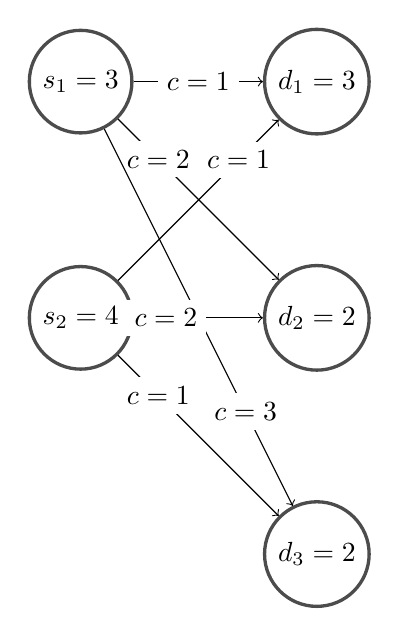
\begin{tikzpicture}[
node/.style={circle, draw=black!70, fill=white!5, very thick, minimum size=9mm}
]
%Nodes
\node[node]      (s1)                                        {$s_1= 3$};
\node[node]      (s2)     [below of =s1, yshift= -2cm]       {$s_2 = 4$};
\node[node]      (d1)     [right of =s1 , xshift= 2cm]       {$d_1 = 3$};
\node[node]      (d2)     [below of = d1, yshift= -2cm]       {$d_2 = 2$};
\node[node]      (d3)     [below of = d2, yshift= -2cm]      {$d_3 = 2$};
%Lines
\draw[->] (s1) -- (d1) node [midway, fill=white] {$c= 1$};
\draw[->] (s1) -- (d2) node [near start, fill=white] {$c = 2$};
\draw[->] (s1) -- (d3) node [near end, fill=white] {$c = 3$};
\draw[->] (s2) -- (d1) node [near end, fill=white] {$c = 1$};
\draw[->] (s2) -- (d2) node [near start, fill=white] {$c = 2$};
\draw[->] (s2) -- (d3) node [near start, fill=white] {$c = 1$};
\end{tikzpicture}
\caption{This picture represents the network for which we will be finding minimum cost flow. The supply and demand nodes are labeled with their corresponding capacities.  The edges between each supply and demand node are labeled according to their cost. To make the problem easier, you can assume all edges have unlimited capacity meaning suppliers can send as much goods as they want over them.}
\label{fig:example1}
\end{framed}
\end{figure}

\begin{figure}
\centering
\begin{framed}
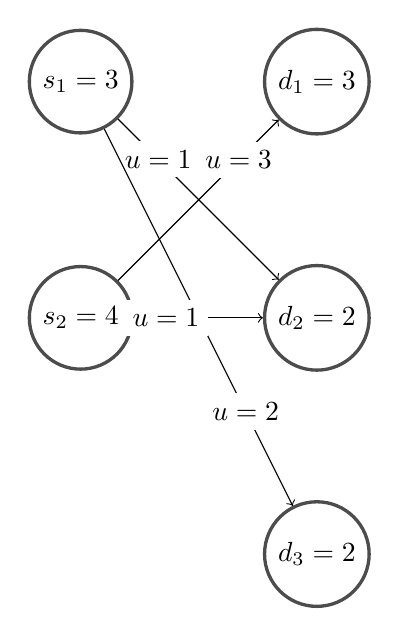
\begin{tikzpicture}[
node/.style={circle, draw=black!70, fill=white!5, very thick, minimum size=9mm}
]
%Nodes
\node[node]      (s1)                                        {$s_1= 3$};
\node[node]      (s2)     [below of =s1, yshift= -2cm]       {$s_2 = 4$};
\node[node]      (d1)     [right of =s1 , xshift= 2cm]       {$d_1 = 3$};
\node[node]      (d2)     [below of = d1, yshift= -2cm]       {$d_2 = 2$};
\node[node]      (d3)     [below of = d2, yshift= -2cm]      {$d_3 = 2$};
%Lines
\draw[->] (s1) -- (d2) node [near start, fill=white] {$u = 1$};
\draw[->] (s1) -- (d3) node [near end, fill=white] {$u = 2$};
\draw[->] (s2) -- (d1) node [near end, fill=white] {$u = 3$};
\draw[->] (s2) -- (d2) node [near start, fill=white] {$u = 1$};
\end{tikzpicture}
\caption{The algorithm starts by matching the capacities on the supply nodes with the capacities on the demand nodes. This is trivial because there are no edge capacities and every node is connected.}
\label{fig:example2}
\end{framed}
\end{figure}

\begin{figure}
\centering
\begin{framed}
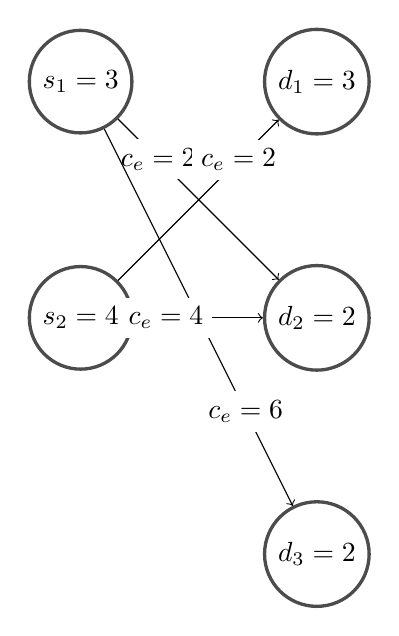
\begin{tikzpicture}[
node/.style={circle, draw=black!70, fill=white!5, very thick, minimum size=9mm}
]
%Nodes
\node[node]      (s1)                                        {$s_1= 3$};
\node[node]      (s2)     [below of =s1, yshift= -2cm]       {$s_2 = 4$};
\node[node]      (d1)     [right of =s1 , xshift= 2cm]       {$d_1 = 3$};
\node[node]      (d2)     [below of = d1, yshift= -2cm]       {$d_2 = 2$};
\node[node]      (d3)     [below of = d2, yshift= -2cm]      {$d_3 = 2$};
%Lines
\draw[->] (s1) -- (d2) node [near start, fill=white] {$c_e = 2$};
\draw[->] (s1) -- (d3) node [near end, fill=white] {$c_e = 6$};
\draw[->] (s2) -- (d1) node [near end, fill=white] {$c_e = 2$};
\draw[->] (s2) -- (d2) node [near start, fill=white] {$c_e = 4$};
\end{tikzpicture}
\caption{This solution is not optimal in terms of cost (yet). I've labled each edge in this figure with the cost each edge has incurred. It works out to 14. The edge costs are just the amount of flow on each edge times its cost.}
\label{fig:example3}
\end{framed}
\end{figure}

\begin{figure}
\centering
\begin{framed}
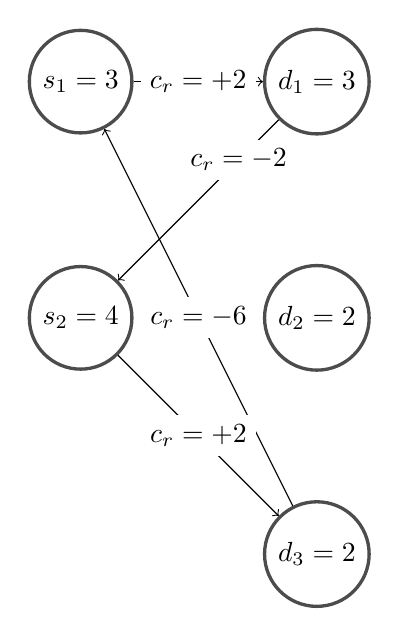
\begin{tikzpicture}[
node/.style={circle, draw=black!70, fill=white!5, very thick, minimum size=9mm}
]
%Nodes
\node[node]      (s1)                                        {$s_1= 3$};
\node[node]      (s2)     [below of =s1, yshift= -2cm]       {$s_2 = 4$};
\node[node]      (d1)     [right of =s1 , xshift= 2cm]       {$d_1 = 3$};
\node[node]      (d2)     [below of = d1, yshift= -2cm]       {$d_2 = 2$};
\node[node]      (d3)     [below of = d2, yshift= -2cm]      {$d_3 = 2$};
%Lines
\draw[->] (s1) -- (d1) node [midway, fill=white] {$c_r=+2$};
\draw[<-] (s1) -- (d3) node [midway, fill=white] {$c_r= -6$};
\draw[<-] (s2) -- (d1) node [near end, fill=white] {$c_r=-2 $};
\draw[->] (s2) -- (d3) node [midway, fill=white] {$c_r=+2$};
\end{tikzpicture}
\caption{In order to improve the cost of flow through the network, we look for a reduced cost cycle. The cycle needs to start and end on the same node. It also needs to alternate between suppliers and demand nodes. This is because you delete costly edges and replace them with less expensive ones. By traversing the cycle we see can reduce the cost by 4 to the optimal amount. Edges in the cycle are labeled with their reduced cost (i.e. how much they improve the total cost)}
\label{fig:example4}
\end{framed}
\end{figure}

\begin{figure}
\centering
\begin{framed}
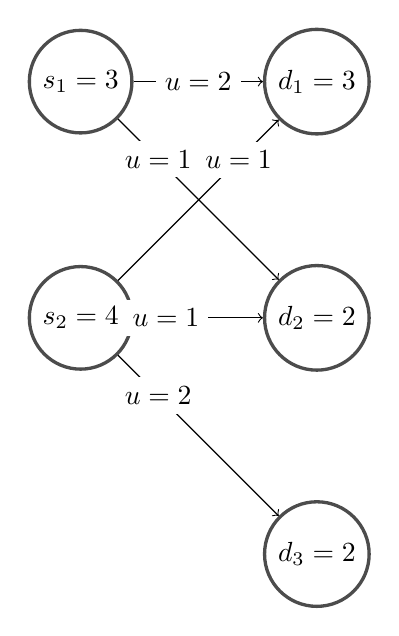
\begin{tikzpicture}[
node/.style={circle, draw=black!70, fill=white!5, very thick, minimum size=9mm}
]
%Nodes
\node[node]      (s1)                                        {$s_1= 3$};
\node[node]      (s2)     [below of =s1, yshift= -2cm]       {$s_2 = 4$};
\node[node]      (d1)     [right of =s1 , xshift= 2cm]       {$d_1 = 3$};
\node[node]      (d2)     [below of = d1, yshift= -2cm]       {$d_2 = 2$};
\node[node]      (d3)     [below of = d2, yshift= -2cm]      {$d_3 = 2$};
%Lines
\draw[->] (s1) -- (d1) node [midway, fill=white] {$u=2$};
\draw[->] (s1) -- (d2) node [near start, fill=white] {$u=1$};
\draw[->] (s2) -- (d1) node [near end, fill=white] {$u=1$};
\draw[->] (s2) -- (d2) node [near start, fill=white] {$u=1$};
\draw[->] (s2) -- (d3) node [near start, fill=white] {$u=2$};
\end{tikzpicture}
\caption{At this point, there are no more reduced cost cycles, so we've found an optimal solution in terms of cost. The edges reflect the amount of units flowing from supply to demand in this solution.}
\label{fig:example5}
\end{framed}
\end{figure}

\begin{figure}
\centering
\begin{framed}
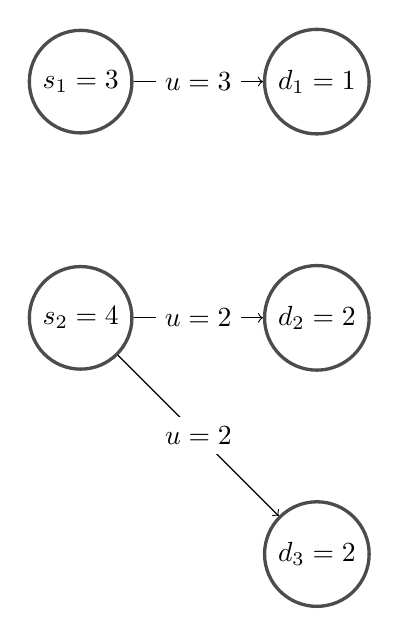
\begin{tikzpicture}[
node/.style={circle, draw=black!70, fill=white!5, very thick, minimum size=9mm}
]
%Nodes
\node[node]      (s1)                                        {$s_1= 3$};
\node[node]      (s2)     [below of =s1, yshift= -2cm]       {$s_2 = 4$};
\node[node]      (d1)     [right of =s1 , xshift= 2cm]       {$d_1 = 1$};
\node[node]      (d2)     [below of = d1, yshift= -2cm]       {$d_2 = 2$};
\node[node]      (d3)     [below of = d2, yshift= -2cm]      {$d_3 = 2$};
%Lines
\draw[->] (s1) -- (d1) node [midway, fill=white] {$u=3$};
\draw[->] (s2) -- (d2) node [midway, fill=white] {$u=2$};
\draw[->] (s2) -- (d3) node [midway, fill=white] {$u=2$};
\end{tikzpicture}
\caption{As long as there aren't minimum cost cycles we've found a solution. Zero-cost cycles exists in this simple network. As a result, there is more than 1 solution that optimizes cost and flow. This figure shows that example.}
\label{fig:example6}
\end{framed}
\end{figure}

\begin{figure}
\centering
\begin{framed}
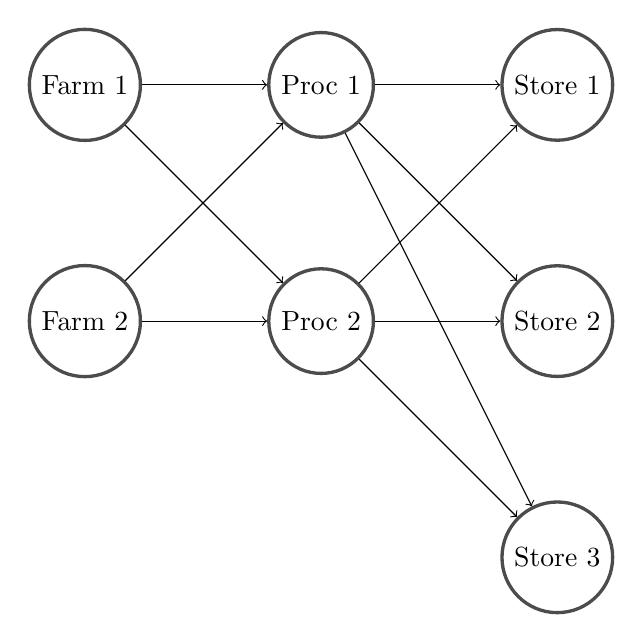
\begin{tikzpicture}[
node/.style={circle, draw=black!70, fill=white!5, very thick, minimum size=9mm}
]
%Nodes
\node[node]      (f1)                                        {Farm 1};
\node[node]      (f2)     [below of = f1, yshift= -2cm]       {Farm 2};
\node[node]      (p1)    [right of = f1, xshift= 2cm]        {Proc 1};
\node[node]      (p2)     [below of =p1, yshift= -2cm]       {Proc 2};
\node[node]      (s1)     [right of = p1 , xshift= 2cm]       {Store 1};
\node[node]      (s2)     [below of = s1, yshift= -2cm]       {Store 2};
\node[node]      (s3)     [below of = s2, yshift= -2cm]      {Store 3};
%Lines
\draw[->] (f1) -- (p1) ;%node [midway, fill=white] {};
\draw[->] (f1) -- (p2) ;%node [near start, fill=white] {};
\draw[->] (f2) -- (p1) ;%node [near start, fill=white] {distance};
\draw[->] (f2) -- (p2) ;%node [midway, fill=white] {distance};
\draw[->] (p1) -- (s1) ;%node [midway, fill=white] {distance};
\draw[->] (p1) -- (s2) ;%node [near start, fill=white] {distance};
\draw[->] (p1) -- (s3) ;%node [near end, fill=white] {distance};
\draw[->] (p2) -- (s1) ;%node [near end, fill=white] {distance};
\draw[->] (p2) -- (s2) ;%node [midway, fill=white] {distance};
\draw[->] (p2) -- (s3) ;%node [near start, fill=white] {distance};
\end{tikzpicture}
\caption{This figure show the structure of the agricultural supply network in my model. Farms grow crops and send their product to intermediate processors. Processors send their product to stores. The processors and farms send their product to the next step in the network using local roads. They choose where to send their crops based on convenience.}
\label{fig:spec}
\end{framed}
\end{figure}

\chapter{Data Sources}

\section{Farms}

In my snapshot of supply, farm's production is proportional to their area. Since, I chose a fairly small geographic region soil, weather, and other elements that effect the production of a crop will not vary greatly. Unless farmers have access to drastically different technologies, the biggest difference affecting yields for farms is the area they've dedicated to growing the crop. I can figure out each farms area by looking at an image created by the National Agricultural Statistical Service \cite{nass}. It is called the Cropland Data Layer. The file is created by measuring the way light reflects off the Earth at certain wavelengths using a satellite called Landsat. The satellite measures this reflection at $30 \times 30$ square meter plots. Based on the reflection is possible to classify point measured by the satellite. The classifications are made using training data from the Farm Service Agency Common Land Unit Program and non-agricultural training data from the United States Geological Survey National Land Cover Dataset 2001. The file forms a grid called a raster. Pixels in the image represent certain crop bands. The accuracy of classification for these pixels isn't great. In Table \ref{tab:band}, you can see how accurate the satellite data is. 

\begin{table}
\centering
\begin{framed}
\begin{tabular}{c|c|c|c|c|c}%
	Type&Band&Correct Pixels&Producer's Accuracy&Kappa&User's Accuracy
    \csvreader[head to column names]{band.csv}{}% use head of csv as column names
    {\\\hline \csvcoli & \csvcolii & \csvcoliii & \csvcoliv& \csvcolv & \csvcolvi}
\end{tabular}
\caption{This table shows the various errors associated with pixels in each crop band in the satellite image \cite{nass}. The pixels are compared with a small test set for accuracy. Correct pixels are the number of pixels extrapolated from the training data. Producer's accuracy is a false negative, where pixels of a known class are classified as something other than that class. User's accuracy shows false positives, where pixels are incorrectly classified as a known class when they should have been classified as something else. Kappa index of agreement gives an overall assessment of the accuracy of the classification.}
\label{tab:band}
\end{framed}
\end{table}

Although individual pixels may be unreliable, I am counting on the fact that clusters of pixels do actually correspond to the locations of farms. Since, I was interested in the area taken up by farms, I used a technique called sieving to make the image more uniform and get rid of random pixels. Basically, this technique involves identifying clusters of continuous pixels and dropping the pixels in clusters smaller than a certain size. After creating the sieve, I converted the raster file into vector based polygons to calculate the area of each cluster and the centroid. Each cluster of continuous pixels became a farm with an area and a centroid. To give you a sense of what farms looked like across the various bands I've included Figure \ref{tab:farms}. You can see how farms for each band look (and how an explanation of how the shapes related to the results) in the results section.


\begin{table}
\centering
\begin{framed}
\begin{tabular}{c|c|c|c|c|c}%
	Band&Total&Average&Minimum&Maximum&Variance
    \csvreader[head to column names]{farms.csv}{}% use head of csv as column names
    {\\\hline \csvcoli & \csvcolii & \csvcoliii & \csvcoliv& \csvcolv & \csvcolvi}
\end{tabular}
\caption{This table is meant to summarize some statistics of interest about the size of farms. Some take aways are that onions (band 49) take up the most area followed by grapes (band 69). Cabbages (band 243) have the smallest range of sizes, but the highest variance within that range. Cherries (band 66) have the smallest variance and the smallest total cover.}
\label{tab:farms}
\end{framed}
\end{table}

\section{Agricultural Dealers}

In order to include intermediate processors (i.e. the agricultural product dealers) into the problem, I used the data on permits from the NYS Department of Agricultural Markets \cite{dam}. Basically, the state keeps a list of all the businesses that buy more than 10,000 dollars in agricultural products. The data set had information about the crops they sold, and their location as an address. I converted the addresses to a spatial coordinate using Nominatim, an open source platform for geolocating (i.e. converting addresses into coordinates). There are roughly 300 of them, but only half were relevant to my problem because they sold the right type of crop. I've included Table \ref{tab:procs} to give you a sense of how many processors were associated with each crop band.

I've included the processors in the problem for two reasons. For starters, they make the problem more realistic by adding limitations to where the farms can sell product. I made sure to choose bands where (for the most part) produce isn't drastically altered during intermediate processing. If the crops make it to these dealers they are going to be sold to stores then consumed. This is because these dealers don't have the necessary permits to use the produce for a purpose other than resale. Only 2 of the 300 processors were from out of state. New York is much bigger on exporting dairy than produce. Obviously, the dealers can sell it to businesses that make prepared foods. For example, a certain percentage of grapes make juices and wine. In practice, the business that with the necessary permits buy in bulk from farms. 

The second reason for including the dealers is because they number of edges to make the problem more computationally tractable. There were roughly 300 licensed agricultural product dealers in the data set. By forcing the edges between stores and farms to the processors, I drastically cut down the number of edges. 

\begin{table}
\centering
\begin{framed}
\begin{tabular}{c|c}%
	Band & Count
    \csvreader[head to column names]{procs.csv}{}% use head of csv as column names
    {\\\hline \csvcoli & \csvcolii}
\end{tabular}
\caption{Grapes (band 69) has the highest number of intermediaries associated with it. The lowest is cherries (band 66).}
\label{tab:procs}
\end{framed}
\end{table}

%stores
\section{Stores}

The data I used on stores came from NYS Division of Food Safety. It is essentially the list of stores that are given health inspections. The store data set has roughly 20,000 different stores, the classifications are based on their permits, their square footage, and their location (as a GPS coordinate). I choose to look at the classification 'JAC' which are vendors that are registered as stores, manufacturers and multiple operations. This is because grocery stores fall under this category. Other categories were not as common and less relevant to selling fresh produce. I've included a map to give a sense of how they are spread through out the state in Figure \ref{fig:map_3}. To get a sense of how the stores vary in size, I've included Table \ref{tab:stores}.

To reflect the fact that a stores might have smaller square footage but face similar demand to other parts of the state, I weight the square footage by the median housing prices. As you can imagine stores in New York City might be the same size as a store upstate, but it you might expect it to sell significantly more produce because the population density is much tighter in New York City and the consumers might have more income to spend. I preform this weighting because I imagine that the stores preform some sort of an optimization problem when choosing how much square footage to buy. If square footage is expensive, it reflects that fact that this location is more lucrative to the store. If stores could sell more produce on inexpensive plots, I would imagine the price would rise. Of course, this is by no means meant to be an exact estimate and specifying a problem where store owners choose optimal square footage to meet demand would be a lot more complicated, it's only supposed to be better than a naive estimate of area by its self.

So as not to have too many edges between the stores and the intermediaries, I've actually aggregated the number of edges by Census district. The reason for using this method to aggregate stores is because I am multiplying square footage of the stores by the property to more appropriately weight the value of the square footage. Also, the census tracts for the most part represent municipalities. As you can imagine. Two stores in the same town probably face the same demand for produce. You can see these weights in Figure \ref{fig:map_4}.

\begin{figure}
\centering
\begin{framed}
\includegraphics[scale=.39]{map_3}
\caption{Here I've mapped all the stores as grey squares. They've been over-layed on top of the census tracts so you can see that stores are spread out between them. You can see are much more sparsely spread in the center of the state.}
\label{fig:map_3}
\end{framed}
\end{figure}

\begin{table}
\centering
\begin{framed}
\begin{tabular}{c|c|c|c|c}%
	Band&Average&Minimum&Maximum&Variance
    \csvreader[head to column names]{stores.csv}{}% use head of csv as column names
    {\\\hline \csvcoli & \csvcolii & \csvcoliii & \csvcoliv & \csvcolv}
\end{tabular}
\caption{This table is meant to convey summary statistics about the characteristics of stores.}
\label{tab:stores}
\end{framed}
\end{table}

\begin{figure}
\centering
\begin{framed}
\includegraphics[scale=.39]{map_4}
\caption{The purpose of this map shows the distribution of median housing values through out the census tracts. The darker the shading, the higher the median property value for that tract. You can see housing is relatively cheap in western and Northern New York, but expensive in the South Western corner of the state.}
\label{fig:map_4}
\end{framed}
\end{figure}

\section{Edge Costs}

In the model, I created an edge between every farm and every processor, and every processor and every store. I measured the cost of traversing this edge as the expected travel time in seconds. In order to find this number, I used open source software called open source routing machine (OSRM). The algorithm that OSRM implements is called contraction hierarchies. Essentially it is a technique to speed up shortest-path routing by first creating precomputed "contracted" versions of the connection graph. Contraction hierarchies can be used to generate shortest-path routes much more efficiently than the standard shortest path algorithm (i.e. Djisktra's). I downloaded a map from the open source mapping project (OSM) and answered routing queries over my local network about routing. I included two tables to give you a sense of some of the summary statistics of the edges. Table \ref{tab:fp_edges} shows the average, minimum, maximum, and variance of edges between farms and product dealers. Table \ref{tab:ps_edges} shows the same thing for the edges between dealers and stores.

\begin{table}
\centering
\begin{framed}
\begin{tabular}{c|c|c|c|c}%
	Band&Average&Minimum&Maximum&Variance
    \csvreader[head to column names]{fp_edges.csv}{}% use head of csv as column names
    {\\\hline \csvcoli & \csvcolii & \csvcoliii & \csvcoliv & \csvcolv}
\end{tabular}
\caption{This table is meant to convey summary statistics about the characteristics of the edges between farms and agricultural product dealers. Grapes (band 69) have the highest variability between edges. }
\label{tab:fp_edges}
\end{framed}
\end{table}

\begin{table}
\centering
\begin{framed}
\begin{tabular}{c|c|c|c|c}%
	Band&Average&Minimum&Maximum&Variance
    \csvreader[head to column names]{ps_edges.csv}{}% use head of csv as column names
    {\\\hline \csvcoli & \csvcolii & \csvcoliii & \csvcoliv & \csvcolv}
\end{tabular}
\caption{This table is meant to convey summary statistics about the characteristics of the edges between farms and agricultural product dealers. The distances are relatively similar to those of between farms and processors, but they are less variable}
\label{tab:ps_edges}
\end{framed}
\end{table}

\chapter{Results}

\section{Overview}

For my project, I asked how the network of farms, agricultural dealers, and store related with transportation prices. To find out, I tracked the movements of certain crops and estimated the cost by optimizing the movement of the crops. By seeing which regions seem to have the highest transportation prices, you can get a much better sense of how to direct future inquiries about how the network and consequently transportation prices effect prices. 

As you would expect, these estimates a lot to do with the concentration of stores, house prices, and the locations of farms. If you are curious about the locations of stores and the and median house prices, you can see them Figures \ref{fig:map_3} and Figure \ref{fig:map_4}.

According to the estimates, prices in Western part of the state are relatively low. This happened because farms are located in this regions and the median house prices are relatively low. There is a lot of supply and little demand.  On the other hand, the South East and the Northern corners of the state are significantly higher. The South East faces the highest prices. This is unsurprising. Property values in this area are high and the concentration of farms is low. That the North would also be high in price was more surprising. Property values are low enough in this region to facilitate farming.  Prices are high here because the agricultural activities that take place are mostly focused on corn and dairy. The farms growing produce are also farthest from the state's northern regions. This is a troubling observation especially when you consider that this region also has some of the lower median incomes in the state. 

You might be wondering why solving the optimization problem was necessary. It seems obvious that your distance from farms and property vales would increase prices for fresh produce. Using the linear program to estimate prices is more tangible and formal way to combine these separate of New York agriculture describe and quantify them. 

Also, there are aspects of the network involved with the linear program that aren't obvious. By estimating prices in the transportation network, certain observation about how the distribution of farms and stores effects costs emerge. It turns out that less obvious properties of the network can effect transportation prices. 

Specifically, more farms smaller in size reduce the variance in relative costs through out the state. This finding is highly related to the structure of the linear program. When you have fewer big farms, the difference in cost between farms will be drastic. If the closest farm does not have enough capacity for all the nearby stores, then stores are forced to chose a farm that is further away incurring higher costs. When the farms are smaller, the difference between the closest farm and the second closest is more gradual. As a result, the difference in prices for the various stores is less pronounced. I noticed this effect in New York state data because it occurs in  prices for cabbage farms. The farms are smaller and more variable in size. As a result, the solution looks different than the other bands.

\section{Visualizing Results}

Understanding over all trends in the linear program isn't obvious. It outputs a list of roughly 8000 prices. In order to glean the key trends, I created tables that summarize key statistics about the linear program's result. Table \ref{tab:county_49}, Table \ref{tab:county_66}, Table \ref{tab:county_69}, and Table \ref{tab:county_243} all summarize the range of possible prices in the linear program for each of the crop bands I chose to analyze. These tables also summarize what county has the highest and lowest prices. As I said before, the counties in the west tend to have the lowest prices. The counties in the South East tend to have the highest prices, followed by the north. The key take aways are that farms are in the Western part of the state, but there is a cluster in the Southern part of the state. As a result, prices according to the linear program should be cheapest in these places. Prices are most expensive in the Northeast corner of the state, followed by the Southeast (i.e. Long Island). Again I want to qualify these statements about prices by saying that prices only represent relative transportation prices. Table  \ref{tab:price_49}, Table  \ref{tab:price_66}, Table  \ref{tab:price_69}, and Table  \ref{tab:price_243} all show basic summary statistics about the mean, and variance of the prices in the linear program solution.

I also visualized the solution to the optimization problem over a map of New York State to make the nature of the network for each crop and the result of the linear program intelligible. The first the images shows the locations of farms based on the crop cover data that was put through the sieve. When you look at the pictures of farms, it becomes obvious how they influenced the solution. Areas around the farms have lower prices. Additionally, the differences in the solutions are explained mostly by the differences in the distribution of the farms throughout the state because  the stores and for the most part dealers stay the same between the various bands in the problem. Figure \ref{fig:farms_49}, Figure \ref{fig:farms_66}, Figure \ref{fig:farms_69}, and Figure \ref{fig:farms_243} show the location of farms for each of the respective crop bands.

The second map I created for each band shows the locations of the farms, stores and dealers on the same map. This is just meant to give a sense of what the network looks like. Farms are represented by pentagons, dealers are stars, and stores are squares. Figure \ref{fig:network_49} , Figure \ref{fig:network_66} , Figure \ref{fig:network_69} , and Figure \ref{fig:network_243} all show how the network looks for each of the respective bands. The final image I created for each band is the most interesting as it actually visualizes the results of the linear program. It shows the various census tracts with shading based on the relative magnitude of the prices. The actually number assigned to the price is some what irrelevant because they only have meaning in relation to each other. They prices reflect the extra time spent on transportation due to including each tract in the network. They are essentially relative costs due to transportation. Figure \ref{fig:prices_49} , Figure \ref{fig:prices_66} , Figure \ref{fig:prices_69} , and Figure \ref{fig:prices_243} all show how the network looks for each of the respective bands.

\section{Comparing Bands}

Obviously, there were differences between the results for each of the bands. Onion prices are unique because there was a cluster of farms in the southern part of the state caused prices to be lower there compared to some of the other bands.


In terms of the various bands Cherries are by far the smallest band in terms of the amount that are sold. Their production is focused in the Western portion of the state. Prices are cheapest by farms and most expensive at the Southeastern and Northeastern parts of the state. The fact that their production is so small and seasonal leads me to question the accuracy of this band. 

The grape farms are concentrated in the Southwestern part of the state. There are some farms in the center of the state and also Eastern Long Island. I included this section because I calculated the edge costs for the grape farms which takes a long time. Truth be told, I don't think that grapes actually are traded using this framework. The supply grown at farms is mostly turned into juices and wines.

Cabbages actually ended up being the most interesting band. The variance in the prices calculated by the algorithm is noticeably lower than any of the other bands as we can see in Table \ref{tab:price_243}. I think this result is more striking in Figure \ref{fig:prices_243}. This result is directly related to the location of the farms through out the state. As I've said before, this is the detail that changes the most between crop bands. Although cabbages are also farmed in the Western portion of the state, they are more spread apart and their size falls within a tighter range. Also, as you can see in Figure \ref{fig:farms_243} there are more individual cabbage farms. At first I suspected that the result was related to the fact that the cabbage farms take up more area, but they actually don't compared to the other bands. Having smaller farms more spread apart seems to have generated this result.

I also provided Table \ref{tab:farm_price} to compare the prices for farms, Table \ref{tab:proc_price} to compare the prices for processors, and Table \ref{tab:store_price} to compare the prices for the various census tracts in each of the bands. Table \ref{tab:farm_county}, Table \ref{tab:proc_county}, and Table \ref{tab:store_county} to compare the information on minimum and maximum counties between the band for farms, dealers and stores.

I also included three images comparing the prices generated at the intermediaries by the linear program for cabbages to onions, cherries, and grapes in Figures \ref{fig:procs_243_49}, Figures \ref{fig:procs_243_66}, and Figures \ref{fig:procs_243_69}. Similarly, I've also included three images comparing the prices generated at the census tracts by the linear program for cabbages to onions, cherries, and grapes in Figures \ref{fig:stores_243_49}, Figures \ref{fig:stores_243_66}, and Figures \ref{fig:stores_243_69}.


\begin{table}
\centering
\begin{framed}
\begin{tabular}{c|c|c|c}%
	Type&Average&Variance&Deviation
    \csvreader[head to column names]{price_49.csv}{}% use head of csv as column names
    {\\\hline \csvcoli & \csvcolii & \csvcoliii & \csvcoliv}
\end{tabular}
\caption{This table shows descriptive statistics about the result of the linear program for onions. You can see that the farms are spread out enough that the program did not need to increase the price at the farms.}
\label{tab:price_49}
\end{framed}
\end{table}

\begin{table}
\centering
\begin{framed}
\begin{tabular}{c|c|c|c|c}%
	Type&Max Price&Max County&Min Price&Min County
    \csvreader[head to column names]{county_49.csv}{}% use head of csv as column names
    {\\\hline \csvcoli & \csvcolii & \csvcoliii & \csvcoliv & \csvcolv}
\end{tabular}
\caption{This table shows the minimum and maximum price for each step in the network according to the linear program for onion. Unsurprisingly, the highest prices were found in the Northeast tip of the state (Clinton County). The minimum was in the center by the most dense cluster of farms.}
\label{tab:county_49}
\end{framed}
\end{table}

\begin{figure}
\centering
\begin{framed}
\includegraphics[scale=.39]{farms_49}
\caption{This table shows the location of onion farms based on the cropland data put through the sieve. If you are interested in descriptive statistics of the farms you can see Table \ref{tab:farms}. You can see there are roughly four clusters of farms. Three of them are in the center of the state, and the fourth is south by Westchester. As you can imagine the locations of farms influenced the prices.}
\label{fig:farms_49}
\end{framed}
\end{figure}

\begin{figure}
\centering
\begin{framed}
\includegraphics[scale=.39]{network_49}
\caption{This figure tries to give you a sense of the onion supply network in New York. The pentagons are farms, the stars are processors, and the squares are stores. Onions had the second highest number of intermediate dealers to choose from as you can see in Table \ref{tab:procs}}
\label{fig:network_49}
\end{framed}
\end{figure}

\begin{figure}
\centering
\begin{framed}
\includegraphics[scale=.39]{prices_49}
\caption{This figure shows the distribution of onion prices through out the state according to the linear program. You can see that the prices are highest in the Northeast and Southeast corners of the state. The fact that there was a cluster of farms in the southern part of the state caused prices to be lower there compared to some of the other bands.}
\label{fig:prices_49}
\end{framed}
\end{figure}


\begin{table}
\centering
\begin{framed}
\begin{tabular}{c|c|c|c}%
	Type&Average&Variance&Deviation
    \csvreader[head to column names]{price_66.csv}{}% use head of csv as column names
    {\\\hline \csvcoli & \csvcolii & \csvcoliii & \csvcoliv}
\end{tabular}
\caption{This table shows descriptive statistics about the result of the linear program for cherries.}
\label{tab:price_66}
\end{framed}
\end{table}

\begin{table}
\centering
\begin{framed}
\begin{tabular}{c|c|c|c|c}%
	Type&Max Price&Max County&Min Price&Min County
    \csvreader[head to column names]{county_66.csv}{}% use head of csv as column names
    {\\\hline \csvcoli & \csvcolii & \csvcoliii & \csvcoliv & \csvcolv}
\end{tabular}
\caption{This table shows the minimum and maximum prices and the counties that they occur for cherries.}
\label{tab:county_66}
\end{framed}
\end{table}

\begin{figure}
\centering
\begin{framed}
\includegraphics[scale=.39]{farms_66}
\caption{This table shows the location of cherry farms based on the cropland data put through the sieve. Cherries had the least amount of area dedicated to them and the farms were scattered throughout the far West portion of the state. If you are interested in descriptive statistics of the farms you can see Table \ref{tab:farms}.}
\label{fig:farms_66}
\end{framed}
\end{figure}

\begin{figure}
\centering
\begin{framed}
\includegraphics[scale=.39]{network_66}
\caption{This figure tries to give you a sense of the cherries supply network in New York. The pentagons are farms, the stars are processors, and the squares are stores. You can see how many dealers there were in Table \ref{tab:procs}}
\label{fig:network_66}
\end{framed}
\end{figure}

\begin{figure}
\centering
\begin{framed}
\includegraphics[scale=.39]{prices_66}
\caption{This figure shows the distribution of cherry prices through out the state according to the linear program. The darker the shading the higher the price. You can see that the prices are highest in the Northeast corner of the state.}
\label{fig:prices_66}
\end{framed}
\end{figure}


\begin{table}
\centering
\begin{framed}
\begin{tabular}{c|c|c|c}%
	Type&Average&Variance&Deviation
    \csvreader[head to column names]{price_69.csv}{}% use head of csv as column names
    {\\\hline \csvcoli & \csvcolii & \csvcoliii & \csvcoliv}
\end{tabular}
\caption{This table shows descriptive statistics about the result of the linear program for grapes.}
\label{tab:price_69}
\end{framed}
\end{table}

\begin{table}
\centering
\begin{framed}
\begin{tabular}{c|c|c|c|c}%
	Type&Max Price&Max County&Min Price&Min County
    \csvreader[head to column names]{county_69.csv}{}% use head of csv as column names
    {\\\hline \csvcoli & \csvcolii & \csvcoliii & \csvcoliv & \csvcolv}
\end{tabular}
\caption{This table shows the minimum and maximum prices and the counties that they occur for grapes.}
\label{tab:county_69}
\end{framed}
\end{table}

\begin{figure}
\centering
\begin{framed}
\includegraphics[scale=.39]{farms_69}
\caption{This table shows the location of grape farms based on the cropland data put through the sieve. If you are interested in descriptive statistics of the farms you can see Table \ref{tab:farms}.}
\label{fig:farms_69}
\end{framed}
\end{figure}

\begin{figure}
\centering
\begin{framed}
\includegraphics[scale=.39]{network_69}
\caption{This figure tries to give you a sense of the grape supply network in New York. The pentagons are farms, the stars are processors, and the squares are stores. You can see how many dealers there were in Table \ref{tab:procs}}
\label{fig:network_69}
\end{framed}
\end{figure}

\begin{figure}
\centering
\begin{framed}
\includegraphics[scale=.39]{prices_69}
\caption{This figure shows the distribution of grape prices through out the state according to the linear program. The darker the shading the higher the price.}
\label{fig:prices_69}
\end{framed}
\end{figure}

\begin{table}
\centering
\begin{framed}
\begin{tabular}{c|c|c|c}%
	Type&Average&Variance&Deviation
    \csvreader[head to column names]{price_243.csv}{}% use head of csv as column names
    {\\\hline \csvcoli & \csvcolii & \csvcoliii & \csvcoliv}
\end{tabular}
\caption{This table shows descriptive statistics about the result of the linear program for cabbages. The variance of the prices is much lower than the other bands. Additionally, the cabbages are more expensive in the Southeast in relatively affluent areas. In the other bands, the crops were more expensive in the Northwest.}
\label{tab:price_243}
\end{framed}
\end{table}

\begin{table}
\centering
\begin{framed}
\begin{tabular}{c|c|c|c|c}%
	Type&Max Price&Max County&Min Price&Min County
    \csvreader[head to column names]{county_243.csv}{}% use head of csv as column names
    {\\\hline \csvcoli & \csvcolii & \csvcoliii & \csvcoliv & \csvcolv}
\end{tabular}
\caption{This table shows the minimum and maximum prices and the counties that they occur for cabbages.}
\label{tab:county_243}
\end{framed}
\end{table}

\begin{figure}
\centering
\begin{framed}
\includegraphics[scale=.39]{farms_243}
\caption{This table shows the location of cabbage farms based on the cropland data put through the sieve. If you are interested in descriptive statistics of the farms you can see Table \ref{tab:farms}.}
\label{fig:farms_243}
\end{framed}
\end{figure}

\begin{figure}
\centering
\begin{framed}
\includegraphics[scale=.39]{network_243}
\caption{This figure tries to give you a sense of the cherries supply network in New York. The pentagons are farms, the stars are processors, and the squares are stores. You can see how many dealers there were in Table \ref{tab:procs}}
\label{fig:network_243}
\end{framed}
\end{figure}

\begin{figure}
\centering
\begin{framed}
\includegraphics[scale=.39]{prices_243}
\caption{This figure shows the distribution of cabbage prices through out the state according to the linear program. The darker the shading the higher the price. The result for cabbages is more spread out across the state than the other bands because of the locations of farms.}
\label{fig:prices_243}
\end{framed}
\end{figure}

\begin{table}
\centering
\begin{framed}
\begin{tabular}{c|c|c|c}%
	Band&Average&Variance&Deviation
    \csvreader[head to column names]{farm_price.csv}{}% use head of csv as column names
    {\\\hline \csvcoli & \csvcolii & \csvcoliii & \csvcoliv}
\end{tabular}
\caption{This table compares the various descriptive statistics for the different farm bands in one place.}
\label{tab:farm_price}
\end{framed}
\end{table}

\begin{table}
\centering
\begin{framed}
\begin{tabular}{c|c|c|c|c}%
	Band&Max Price&Max County&Min Price&Min County
    \csvreader[head to column names]{farm_county.csv}{}% use head of csv as column names
    {\\\hline \csvcoli & \csvcolii & \csvcoliii & \csvcoliv & \csvcolv}
\end{tabular}
\caption{This table compares the minimum and maximum prices between the four crop bands for farms.}
\label{tab:farm_county}
\end{framed}
\end{table}

\begin{table}
\centering
\begin{framed}
\begin{tabular}{c|c|c|c}%
	Band&Average&Variance&Deviation
    \csvreader[head to column names]{proc_price.csv}{}% use head of csv as column names
    {\\\hline \csvcoli & \csvcolii & \csvcoliii & \csvcoliv}
\end{tabular}
\caption{This table compares the various descriptive statistics for the different farm product dealers across the four bands in one place.}
\label{tab:proc_price}
\end{framed}
\end{table}

\begin{table}
\centering
\begin{framed}
\begin{tabular}{c|c|c|c|c}%
	Band&Max Price&Max County&Min Price&Min County
    \csvreader[head to column names]{proc_county.csv}{}% use head of csv as column names
    {\\\hline \csvcoli & \csvcolii & \csvcoliii & \csvcoliv & \csvcolv}
\end{tabular}
\caption{This table compares the minimum and maximum prices between the four crop bands for the intermediate dealers.}
\label{tab:proc_county}
\end{framed}
\end{table}

\begin{figure}
\centering
\begin{framed}
\includegraphics[scale=.39]{procs_243_49}
\caption{This figure compares the difference in prices between onions and cabbages at the intermediaries. I chose cabbages because the result of the linear program was most different for this band. The stars represent the dealers. Darker means onion prices were greater. Lighter means cabbage prices were greater.}
\label{fig:procs_243_49}
\end{framed}
\end{figure}

\begin{figure}
\centering
\begin{framed}
\includegraphics[scale=.39]{procs_243_66}
\caption{This figure compares the difference in prices between cherries and cabbages at the intermediaries. I chose cabbages because the result of the linear program was most different for this band. The stars represent the dealers. Darker means cherry prices were greater. Lighter means cabbage prices were greater.}
\label{fig:procs_243_66}
\end{framed}
\end{figure}

\begin{figure}
\centering
\begin{framed}
\includegraphics[scale=.39]{procs_243_69}
\caption{This figure compares the difference in prices between grapes and cabbages at the intermediaries. I chose cabbages because the result of the linear program was most different for this band. The stars represent the dealers. Darker means grape prices were greater. Lighter means cabbage prices were greater.}
\label{fig:procs_243_69}
\end{framed}
\end{figure}

\begin{table}
\centering
\begin{framed}
\begin{tabular}{c|c|c|c}%
	Band&Average&Variance&Deviation
    \csvreader[head to column names]{store_price.csv}{}% use head of csv as column names
    {\\\hline \csvcoli & \csvcolii & \csvcoliii & \csvcoliv}
\end{tabular}
\caption{This table compares the various descriptive statistics for the different stores across the four bands in one place.}
\label{tab:store_price}
\end{framed}
\end{table}

\begin{table}
\centering
\begin{framed}
\begin{tabular}{c|c|c|c|c}%
	Band&Max Price&Max County&Min Price&Min County
    \csvreader[head to column names]{store_county.csv}{}% use head of csv as column names
    {\\\hline \csvcoli & \csvcolii & \csvcoliii & \csvcoliv & \csvcolv}
\end{tabular}
\caption{This table compares the minimum and maximum prices between the four crop bands for the different census tracts}
\label{tab:store_county}
\end{framed}
\end{table}

\begin{figure}
\centering
\begin{framed}
\includegraphics[scale=.39]{stores_243_49}
\caption{This figure compares the difference in prices between onions and cabbages at the census tracts. I chose cabbages because the result of the linear program was most different for this band. The stars represent the dealers. Darker means onion prices were greater. Lighter means cabbage prices were greater.}
\label{fig:stores_243_49}
\end{framed}
\end{figure}

\begin{figure}
\centering
\begin{framed}
\includegraphics[scale=.39]{stores_243_66}
\caption{This figure compares the difference in prices between cherries and cabbages at the census tracts. I chose cabbages because the result of the linear program was most different for this band. The stars represent the dealers. Darker means cherry prices were greater. Lighter means cabbage prices were greater.}
\label{fig:stores_243_66}
\end{framed}
\end{figure}

\begin{figure}
\centering
\begin{framed}
\includegraphics[scale=.39]{stores_243_69}
\caption{This figure compares the difference in prices between grapes and cabbages at the census tracts. I chose cabbages because the result of the linear program was most different for this band. The stars represent the dealers. Darker means grape prices were greater. Lighter means cabbage prices were greater.}
\label{fig:stores_243_69}
\end{framed}
\end{figure}

\chapter{Discussion}

\section{Robustness of Solutions}

%complementary slackness
From an economic perspective, I would hope you are skeptical of any solution to this problem involving prices found by the simplex algorithm. Optimal transportation can have more than one possible solution. The example I've worked out the problem actually has more than one solution and I've demonstrated it in Figure \ref{fig:example6}. The question becomes how do I know when I've found all possible minimum cost flow distributions through the network with the simplex algorithm. Perhaps I got lucky and found an interesting solution with certain properties that aren't robust.

Luckily, linear programming has a property that allows me to characterize all possible solutions. This property is called complementary slackness and it says that the optimal value of the primal and the dual objective functions will be equivalent. The intuition behind this idea is relatively easy to show with some matrix algebra.

Very generally speaking a linear program has the primal form

$$\text{Maximize } c' x$$
$$\text{Subject to}$$
$$Ax \leq b$$

And, it's corresponding dual would be

$$\text{Minimize } y' b$$
$$\text{Subject to}$$
$$A'y \leq c$$

We can massage the objective function to see that the values of the primal and dual objective functions will be the same

$$(A'y)' \leq c'$$
$$ y'A \leq c'$$
$$ y'Ax \leq c'x$$
$$y' b \leq c'x$$

In the same vain, 

$$ Ax \leq b$$
$$ y'Ax \leq y'b$$
$$ (yA')'x \leq c'x$$
$$ c'x \leq  y' b $$

As consequence of these two observations we know the objective functions must take the same value.

$$c'x = y' b$$

By this logic the objective function for any solution to the primal or dual problem will be the same. You can use this idea to check how robust certain properties of your solution are by limiting the linear program with the value of the objective function as a constraint. 

For example, in regards to the transportation if you want to check to see whether your maximum price $p = p^{max}$ is only particular to your solution, you can add constraint extra constraints to your original problem to test this. You can request that one of the prices exceeds the maximum, $p > p^{max}$ to check this property of the solution. And, in order to ensure that this is still a valid solution to the original problem you can limit the value of your objective function. If the value of the objective was $c^*$ then you can add the constraint  $ \sum_{d \in D}  (\text{demand at } d) \cdot p_{d} -   \sum_{s \in S}  (\text{supply at } s) \cdot p_{s} = c^*$

For each of the bands, I tried to find an alternate solutions to the linear program in four ways using complementary slackness. Essentially, I parsed the value of the objective function from the solution file and added it as a constraint. Then I added constraints that tried pushing the maximum price to be higher or lower than it was in the original solution. I also tried pushing the minimum price to be lower or higher than it was in the solution. I was able to change get a second solution across all bands. This sheds doubt on my solution, but the differences weren't drastic. The over arching properties held. In fact, in each file at most 500 prices of the roughly 8000 prices across farms and stores changed. Most importantly the minimum and maximum values didn't change by more than 10 percent. I can provide the differences as a .csv file upon request. They can also be generated using the git repository. They are rather cumbersome (there are 16 of them, each with between 50 and 500 lines).

To be honest, I think the changes in the solution has more to do with rounding errors related to the way that python stores floating point numbers rather than actual differences to the solution. When the value of the objective function is parsed from the solution file into a python float the last decimal point may not be accurate. In fact, in all cases the objective function value was not exactly accurate. This would absolutely explain why the solutions were different.

%Transportation problem discussion

%Discusion
\section{Conclusion}
Before settling on just looking at transportation costs in relation to the network, I tried answering how the network of farms, dealers, and stores relate to prices and consumer behavior. I thought moving from farms to stores within the network would incur transportation costs would in turn translate into higher prices. I only got as far as analyzing how the network determined transportation costs. However, there is more to this subquestion than you would expect. Transportation costs offer the best glimpse at how the network structure effects prices and nutritional outcomes. The framework of optimal transportation applies surprisingly in explain the mechanism by which the network determines the transportation costs in New York. Although transportation cost are not the full picture, they are the best possible view at how the network influences prices which has implications in nutrition and industrial organization.

Depending upon how transportation costs influence prices for these various types of produce, the implications of this project are large. The literature establishes that prices are key in determining nutritional outcomes. Since, transporting food to the Northeast and Southeastern corners of the state is difficult one might worry about nutritional outcomes in those regions. More expensive prices on Long Island and New York city reflects the higher cost of living in those areas. However, the observations about the Northern tip of the state are troubling. If transportation costs influence prices then it raises alarm about areas with high costs in the Northern parts of the state. These regions have low median incomes, but high prices. This project also formalizes the intuition that scattering smaller farms through out the state provides more options which in turn make it easier to transport produce to various parts of the state.

The way that prices are effected by the structure of the network of farms, processors, and stores is a theoretical question about how the network of firms in this industry determines prices.  Obviously, there are factors that determine price that are outside of transportation costs. It seems logical that transportation costs would increase prices. In the context that I've chosen, transportation costs are incredibly relevant. The market being small and self contained means that production is relatively similar between farms. You could even increase all of the prices by a similar amount if you wanted to reflect these other production costs. Going back to the problem definition, since $p$ are slack variables, you can actually increase all the prices by the same amount and still have a solution that encouraged optimal transportation. Of course, this solution would lie on the same manifold as the original one. The reason I am not entirely positive that transportation costs influence prices is because of the stores are not as self contained as the farms. A lot of these stores are part of national chains. Perhaps decisions that are optimal for the business on a national scale do not seem optimal on a local level in terms of which farms and dealers the store decides to get its produce from. For example, one grocery chain might decide to work with only one agricultural dealer even though from the perspective of transportation costs, it would be beneficial to work with two.

Although predicting prices through transportation costs is circuitous, it offers the best possible view of how the network structure effects prices and nutritional outcomes. How the network effects prices is a theoretical question. A statistical model could not answer how the network related to prices. In order to quantify a statistical relationship between the network of farms, stores, and dealers and prices, the statistical model would need vectors as inputs. Your result would be more about the property of the network you choose to look at and not about the entire network its self. You could always find some other property of the network to compare with prices that might seem important or might seem irrelevant in a statistical context. For example, if it turned out that actual prices in a given region were correlated with the result of the linear program, it wouldn't tell you anything about whether transportation costs effect prices and consumer behavior. All it would tell you is that some aspect of the structure was related to the price. It wouldn't tell anything about what aspect was important though, because there are so many ways to represent the network in the regression. Perhaps as a future project, I will build a more fleshed out mechanism for relating the transportation costs with prices.

You can criticize the transportation costs because they are not perfect estimations. You can argue prices in the problem only reflect linear transportation costs. For example, it is possible that the extra cost involved with shipping goods to the Northern corners of the state may only be logarithmic with travel time. There is the issue of exports and crops used for other purposes. I mentioned it a few times, but the Grape band data is almost completely useless. I took the time to load it into the database and calculate the edge costs so I figured I show what I found. That being said, for all these bands some proportion can be sent out of state our bought by business that won't sell it fresh. For this reason, I am under-estimate costs. If I could adding demand for sales to manufacturers and inter-state exports it would increase prices. That being said, the estimated prices are still economically significant without exports. They represent a minimum for prices; adding additional demand from out-of-state increases costs in-state. Additionally, most of the categories of produce have a short shelf life and are exported in insignificant quantities with the exception of apples. All this being said, I think the crops I chose to analyze are being transported short enough distances in small enough quantities that I do not have to worry about a non-linear cost structure or a complicated existing infrastructure designed to transport the crops.

Another issue is that the data I used is wrong. Census data about median income isn't available for certain census tracts. There are always problems with classifying crops using satellite bands as I discussed before. As I said, I used a sieve to try to remove extraneous pixels that were misclassified. CAdditionally, consumers preferences in various regions might not be reflected in cost of square footage. Perhaps square footage is cheap, but consumers buy a lot of produce proportionally in the state. I find this a little far fetched. I would imagine preferences for produce do not vary drastically over such a small region and such commonly used crops like cabbage, onions are cherries. Finally, there might be smaller farm dealers that don't have to register with the Department of Agricultural Markets because they sell less than 10,000 a year in goods. This would change the nature of the network. Still, data is never perfect. No mater what data I used, there would be room for improvement. Despite these reservations the data paints a surprisingly detailed picture of agricultural markets in New York. 

So to conclude, my project tries to explain how the network of farms, stores, and agricultural dealers relates to the cost of moving produce through the state. Transportation costs offer the best glimpse at how the network structure effects prices and nutritional outcomes.  The crops I've chosen seem to be a surprising analogue for optimal transportation. The snapshot I have about the farms, dealers, and stores are surprisingly well suited for this analysis.  Optimal transportation is a reasonable frame for onions, cherries, grapes, and cabbages in New York state. It seems self evident that this economic knowledge effects firms decision making process. It is the best possible glimpse at how the network reflects prices. The literature seems to agree that higher prices for nutritionally sound foods generally relates to worse outcomes, especially when the prices are complemented with information about what to buy. Finally, it takes into account the broader set of circumstances that may effect nutritional outcomes. 

\pagebreak

\begin{thebibliography}{99}
\bibitem{Bernell}Bernell, S., Weber, B., {\&} Edwards, M. (2006). Restricted Opportunities, Personal Choices, Ineffective Policies: What Explains Food Insecurity in Oregon? Journal of Agricultural and Resource Economics, 31(2), 193-211. 
\bibitem{Chung} Chung, Chanjin, and Samuel L. Myers. "Do the Poor Pay More for Food? An Analysis of Grocery Store Availability and Food Price Disparities." The Journal of Consumer Affairs 33.2 (1999): 276-96.
\bibitem{Cook} Cook, W. J., Cunningham, W. H., Pulleyblank, W. R.,  {\&}  Schrijver, A. (1998). Combinatorial optimization (pp. 91-126). New York: John Wiley  {\&}  Sons.
\bibitem{Hwang} Hwang, M., {\&} Smith, M. (2012). Integrating publicly available web mapping tools for cartographic visualization of community food insecurity: A prototype. GeoJournal, 77(1), 47-62.
\bibitem{Just} Just, R., {\&} Weninger, Q. (1997). Economic Evaluation of the Farmers' Market Nutrition Program. American Journal of Agricultural Economics, 79(3), 902-917.
\bibitem{dfs} NYS Division of Food Safety {\&} Inspection (2016). Retail Food Stores [Download table]. Retrieved from \url{https://data.ny.gov/Economic-Development/Retail-Food-Stores/9a8c-vfzj}
\bibitem{dam} NYS Department of Agriculture and Markets (DAM) (2016). Farm Product Dealer Licenses Currently Issued [Download table]. Retrieved from \url{https://data.ny.gov/Economic-Development/Retail-Food-Stores/9a8c-vfzj}
\bibitem{Larson} Larson, J., {\&} Moseley, W. (2012). Reaching the limits: A geographic approach for understanding food insecurity and household hunger mitigation strategies in Minneapolis-Saint Paul, USA. GeoJournal, 77(1), 1-12.
\bibitem{Stewart} Stewart, T., {\&} Ittmann, H. (1979). Two-Stage Optimization in a Transportation Problem. The Journal of the Operational Research Society, 30(10), 897-904.
\bibitem{census} U.S. Census Bureau. (2011). American Community Survey, 2010 ACS 5-year Selected Population Tables [Table B25077]. Retrieved from \url{https://factfinder.census.gov/faces/nav/jsf/pages/download_center.xhtml}
\bibitem{nass3} USDA, NASS. (2012) Census Publications Market Value of Ag Products. Retrieved from \url{https://www.agcensus.usda.gov/Publications/2012/Online_Resources/Rankings_of_Market_Value/New_York/}
\bibitem{nass} USDA, NASS. (2011). USDA National Agricultural Statistics Service 2010 New York Cropland Data Layer [Download]. Retrieved from \url{http://cugir.mannlib.cornell.edu/bucketinfo.jsp?id=8033}
\bibitem{nass2} USDA, NASS. (2015) QuickStat Searchable Database. [New York State, Fruit and Tree Nuts, Vegetables, Cherries, Onions, Cabbages, Grapes]. Retrieved from \url{https://www.nass.usda.gov/Statistics_by_State/New_York/}

\end{thebibliography}



\end{document}